\begin{answer}

  The number of trials needed without changing the seed is 60.
  
  \color{Comments}We noticed that different but mathematically equivalent implementations on choosing random action in function $\mathsf{choose\_action}$ will result different plots. We have three basic examples here, but there may be more possibilities. The plot below uses
  \begin{verbatim}
  action = 0 if np.random.uniform() < 0.5 else 1
  \end{verbatim}

  \begin{center}
    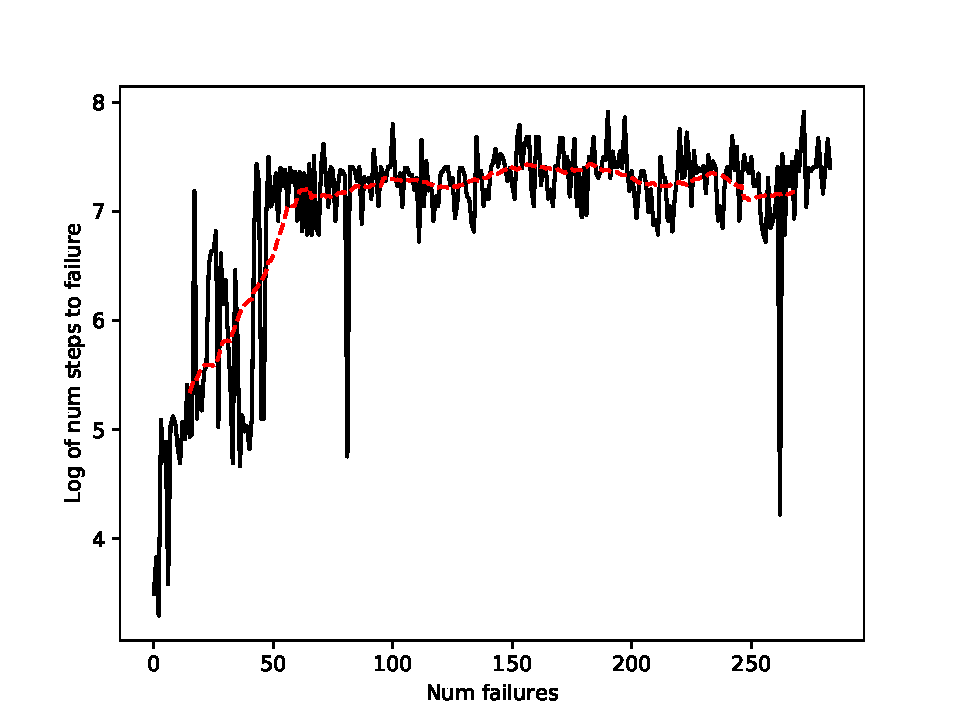
\includegraphics[width=6cm]{../src/cartpole/control_case1.pdf}
  \end{center}

  The plot below uses
  \begin{verbatim}
  action = 0 if np.random.uniform() >= 0.5 else 1
  \end{verbatim}
  \begin{center}
  	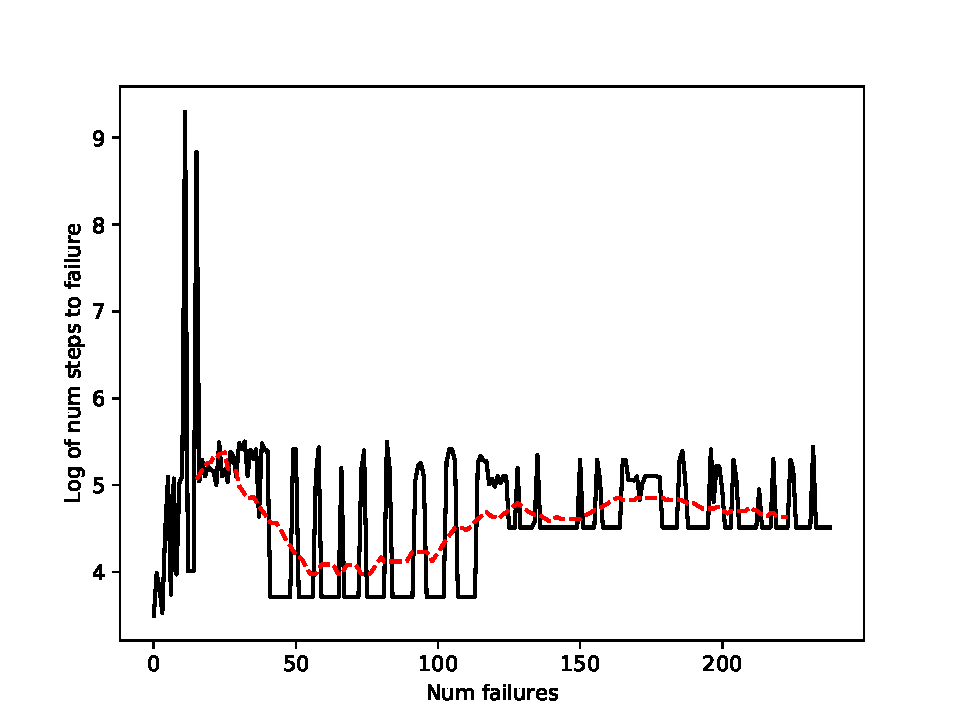
\includegraphics[width=6cm]{../src/cartpole/control_case2.pdf}
  \end{center}

  The plot below uses
  \begin{verbatim}
  action = np.random.choice([0, 1])
  \end{verbatim}
  \begin{center}
  	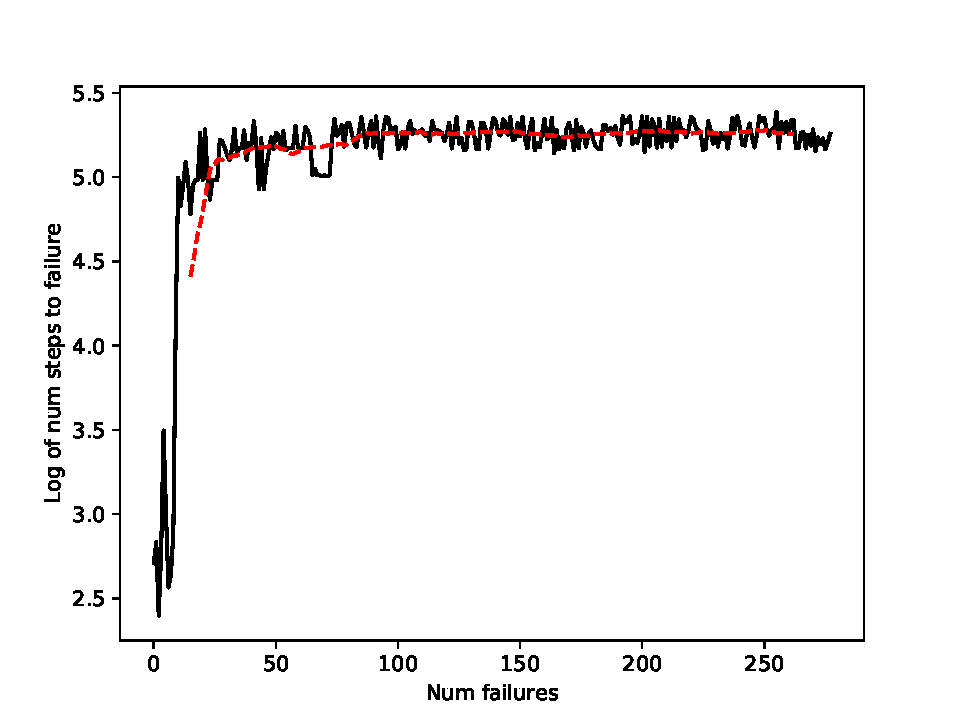
\includegraphics[width=6cm]{../src/cartpole/control_case3.pdf}
  \end{center}

\end{answer}
